\subsection{Постановка задач}
Найти стабильную конформацию (equilibrium state, ES) молекулы трифторметанол методом B3LYP/6-31G, проведя оптимизацию исходной геометрии. Предложить вид переходного состояния (transition state, TS) в барьере поворота вокруг C-O-связи. Провести оптимизацию переходного состояния методом B3LYP/6-31G и привести следующие результаты:
\begin{itemize}
    \item[-] энергия ES и TS и вклады в них;
    \item[-] высота потенциального барьера;
    \item[-] определить, может ли этот барьер преодолеваться термически при комнатной температуре.
\end{itemize}

\begin{figure}[H]
\centering
\captionsetup{justification=centering}
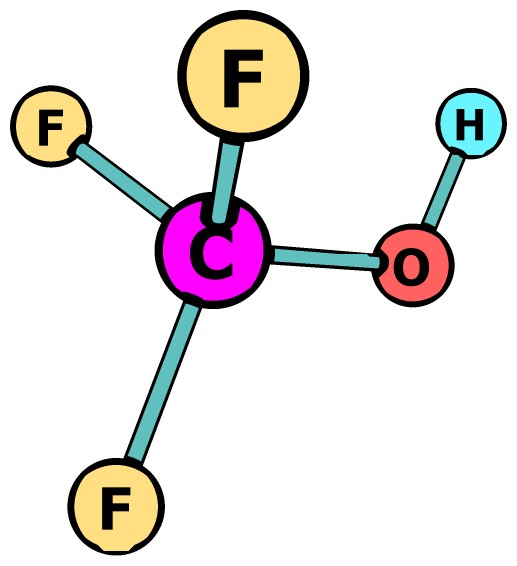
\includegraphics[scale=0.4]{fig/0.jpg}
\caption{Молекулы трифторметанол}
\end{figure}